
\subsection{Implementation details}
In this section we compare the decomposition algorithm (both with QLS and ELS) against SNOPT \cite{snopt}.
The decomposition algorithm is written in \textit{Python 2.7} while we use the official Python interface for SNOPT. We also use \texttt{numpy} library, linked with \texttt{blas} and \texttt{ATLAS} libraries. The PC used for the experiments is equipped with and Intel i7 3630QM processor, 8GB of RAM and a Linux based distribution.\\

\subsection{Test problems and stopping criterion}
In all the following experiments we used the NASDAQ-2196 dataset\footnotemark[1]; from the covariance matrix contained in the dataset, we compute the correlation matrix and we use that instead of the covariance one for numerical reasons. 
\footnotetext[1]{NASDAQ-2196 dataset can be downloaded at \url{http://host.uniroma3.it/docenti/cesarone/datasetsw3_tardella.html}}
In order to obtain comparable results, in our scheme we use a \textit{stop criterion} that is the same used by SNOPT, i.e. we stop the algorithm when
\begin{equation}\label{eq:stop}
\left| \frac{\partial f(x^k,y^k)}{d{x_{j(k)}}} - \frac{\partial f(x^k,y^k)}{d{x_{i(k)}} }\right| < \epsilon
\end{equation}
In SNOPT, this is (almost) equivalent to set the \texttt{Major optimality tolerance} optional parameter to $\epsilon$. 

\subsection{Numerical results}
\subsubsection{General box constraints}
In this section we use different combinations for the box constraints $l$ and $u$ and we compare the values assumed by the objective function in the critical point reached by the different algorithms. In these tests we take:
\begin{equation}
x_i^0 = \frac{1}{n} \quad \forall i \in \{1, .., n \}
\end{equation}
We denote with $x_{D}$ the solution produced by the decomposition algorithm and with $x_{S}$ the solution produced by SNOPT. In Figure (\ref{fig:box}), we compare the value of $f(x_{D})$ with $f(x_{S})$ using different box constraints when the two algorithms converges at two different critical points.

\begin{figure}
\makebox[\textwidth][c]{

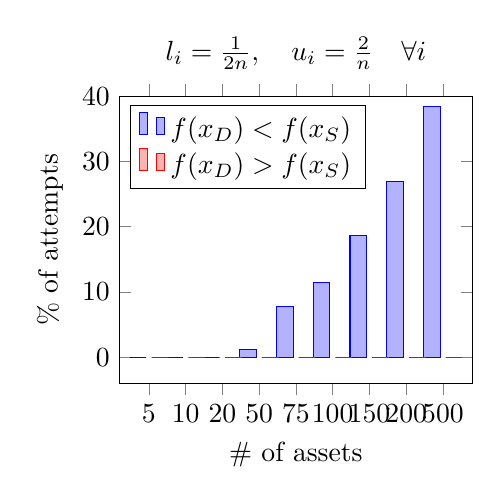
\begin{tikzpicture}
\begin{axis}[%
ybar,
xlabel={\# of assets},
ylabel={\% of attempts},
ylabel near ticks,
legend pos=north west,
symbolic x coords = {5,10,20,50,75,100,150,200,500},
bar width=6pt,
xtick=data,
ymax=40,
width=.5\textwidth,
title={$l_i = \frac{1}{2n}, \quad u_i = \frac{2}{n} \quad \forall i$},
]
\addplot coordinates { 
(5,0)         
(10,0)
(20,0)
(50,1.2)
(75,7.8)
(100,11.5)
(150,18.7)
(200,26.9)
(500,38.4)
 };
 
 \addplot coordinates { 
(5,0)         
(10,0)
(20,0)
(50,0)
(75,0)
(100,0)
(150,0)
(200,0)
(500,0)
 };

\addlegendentry{$f(x_{D}) < f(x_{S})$}
\addlegendentry{$f(x_{D}) > f(x_{S})$}
\end{axis}
\end{tikzpicture}


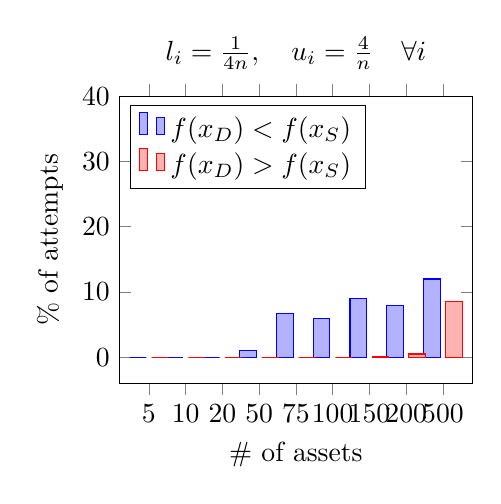
\begin{tikzpicture}
\begin{axis}[%
ybar,
xlabel={\# of assets},
ylabel={\% of attempts},
ylabel near ticks,
legend pos=north west,
symbolic x coords = {5,10,20,50,75,100,150,200,500},
bar width=6pt,
xtick=data,
ymax=40,
width=.5\textwidth,
title={$l_i = \frac{1}{4n}, \quad u_i = \frac{4}{n} \quad \forall i$}
]
\addplot coordinates { 
(5,0)         
(10,0)
(20,0)
(50,1.0)
(75,6.7)
(100,6.0)
(150,9.0)
(200,7.9)
(500,12.0)
 };
 
 \addplot coordinates { 
(5,0)         
(10,0)
(20,0)
(50,0)
(75,0)
(100,0)
(150,0.1)
(200,0.5)
(500,8.6)
 };

\addlegendentry{$f(x_{D}) < f(x_{S})$}
\addlegendentry{$f(x_{D}) > f(x_{S})$}
\end{axis}
\end{tikzpicture}
}

\makebox[\textwidth][c]{
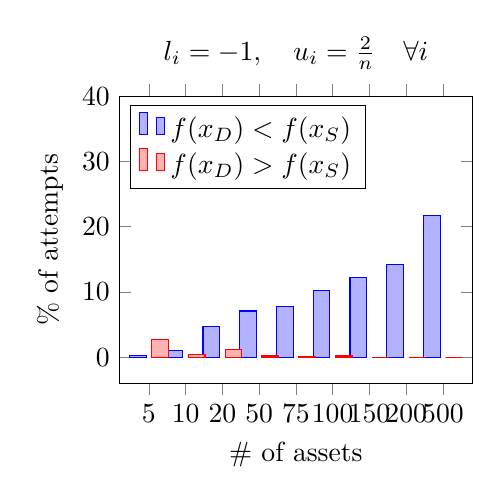
\begin{tikzpicture}
\begin{axis}[%
ybar,
xlabel={\# of assets},
ylabel={\% of attempts},
ylabel near ticks,
legend pos=north west,
symbolic x coords = {5,10,20,50,75,100,150,200,500},
bar width=6pt,
xtick=data,
ymax=40,
width=.5\textwidth,
title={$l_i = -1, \quad u_i = \frac{2}{n} \quad \forall i$}
]
\addplot coordinates { 
(5,0.3)         
(10,1.0)
(20,4.7)
(50,7.1)
(75,7.8)
(100,10.2)
(150,12.2)
(200,14.2)
(500,21.7)
 };
 
 \addplot coordinates { 
(5,2.7)         
(10,0.4)
(20,1.2)
(50,0.2)
(75,0.1)
(100,0.2)
(150,0)
(200,0)
(500,0)
 };

\addlegendentry{$f(x_{D}) < f(x_{S})$}
\addlegendentry{$f(x_{D}) > f(x_{S})$}
\end{axis}
\end{tikzpicture}
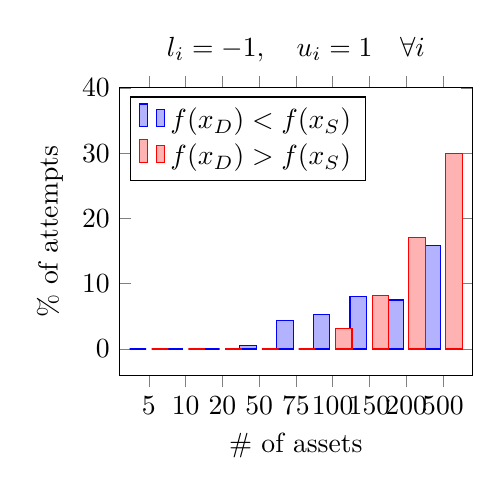
\begin{tikzpicture}
\begin{axis}[%
ybar,
xlabel={\# of assets},
ylabel={\% of attempts},
ylabel near ticks,
legend pos=north west,
symbolic x coords = {5,10,20,50,75,100,150,200,500},
bar width=6pt,
xtick=data,
ymax=40,
width=.5\textwidth,
title={$l_i = -1, \quad u_i = 1 \quad \forall i$}
]
\addplot coordinates { 
(5,0)         
(10,0)
(20,0)
(50,0.6)
(75,4.4)
(100,5.3)
(150,8.0)
(200,7.5)
(500,15.9)
 };
 
 \addplot coordinates { 
(5,0)         
(10,0)
(20,0)
(50,0)
(75,0)
(100,3.2)
(150,8.2)
(200,17.1)
(500,30)
 };

\addlegendentry{$f(x_{D}) < f(x_{S})$}
\addlegendentry{$f(x_{D}) > f(x_{S})$}
\end{axis}
\end{tikzpicture}
}
\caption{Comparison of objective function values for $x_{D}$ and $x_{S}$ with different box constraints. For each $n$ we perform $1000$ experiments for both the algorithms.}
\label{fig:box}
\end{figure}

In Figure (\ref{subfig-1:time1}) we compare the average execution time of the decomposition algorithm (with inexact and exact line search) against SNOPT using 
\begin{equation}
x^0_i = \frac{1}{n} \quad \forall i
\end{equation}
and 
\begin{equation}\label{eq:generalbox}
l_i = \frac{1}{2n} \quad \forall i \qquad u_i = \frac{2}{n}  \quad \forall i
\end{equation} 
The $\epsilon$ in the stop criterion (\ref{eq:stop}) is set to $10^{-10}$. In Figure (\ref{subfig-2:iterations1}) we compare the average number of iterations performed by the decomposition algorithm using the two different strategies for step computation (inexact and exact).
\begin{figure}
\makebox[\textwidth][c]{
\subfloat[Comparison of average execution time \label{subfig-1:time1}]{%
\begin{tikzpicture}
\begin{axis}[%
xlabel={\# of assets},
ylabel={Exe Time (s)},
legend pos=north west,
ylabel near ticks,
width=.5\textwidth
]
\addplot [color=blue,solid,mark=x,mark options={solid}]
  table[row sep=crcr]{%
100	.105\\
200	.214\\
300	.340\\
500	.737	\\
750	1.713		\\
1000 3.303 \\
1250 5.400 \\
1500 9.58\\
};


\addplot [color=red,solid,mark=x,mark options={solid}]
  table[row sep=crcr]{%
100	 .068   \\
200	 .158	\\
300	 .258	\\
500	 .620	\\
750	 1.54	\\
1000 3.42  \\
1250 6.24\\
1500 10.93 \\
};


\addplot [color=gr,solid,mark=x,mark options={solid}]
  table[row sep=crcr]{%
100	.005	\\
200	.014	\\
300	.035	    \\
500	.118	    \\
750	 .286  \\
1000 0.561	\\
1250 0.824	\\
1500 1.43 \\
};

\addlegendentry{DEC$_{(ELS)}$}
\addlegendentry{DEC$_{(QLS)}$}
\addlegendentry{SNOPT}
\end{axis}
\end{tikzpicture}
}
\hfill
\hspace{1em}\subfloat[Comparison of average iterations\label{subfig-2:iterations1}]{%
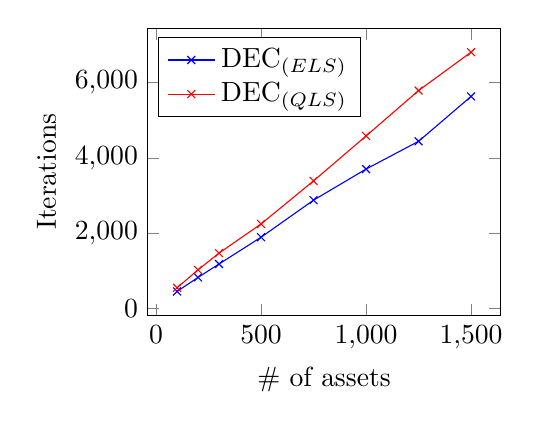
\begin{tikzpicture}
\begin{axis}[%
xlabel={\# of assets},
ylabel={Iterations},
legend pos=north west,
ylabel near ticks,
width=.5\textwidth
]
\addplot [color=blue,solid,mark=x,mark options={solid}]
  table[row sep=crcr]{%
100	445 \\
200	819 \\
300	1176 \\
500	1888\\
750	2874 \\
1000	 3701\\
1250	 4439\\
1500 5634\\
};

\addplot [color=red,solid,mark=x,mark options={solid}]
 table[row sep=crcr]{%
100	543    \\
200	1021	\\
300	1466	\\
500	2241	\\
750	3387	\\
1000	 4582	\\
1250	 5789	\\
1500	 6811\\
};

\addlegendentry{DEC$_{(ELS)}$}
\addlegendentry{DEC$_{(QLS)}$}
\end{axis}
\end{tikzpicture}
}
}
\caption{Comparison of performances using $\epsilon = 10^{-10}$ in (\ref{eq:stop}) with box constraints defined in (\ref{eq:generalbox})}
\end{figure}

\subsubsection{Classical box constraints}
In this section we use 
\begin{equation}\label{eq:classicalbox}
l_i = 0 \quad \forall i \qquad u_i = 1  \quad \forall i
\end{equation} 
In Figure (\ref{subfig-1:time2}) we compare the average execution time of the decomposition algorithm (with inexact and exact line search) against SNOPT using 
\begin{equation}
x^0 = [1, 0, .., 0]
\end{equation}
The $\epsilon$ in the stop criterion (\ref{eq:stop}) is set to $10^{-10}$. In Figure (\ref{subfig-2:iterations2}) we compare the average number of iterations performed by the decomposition algorithm using the two different strategies for step computation (inexact and exact).
\begin{figure}
\makebox[\textwidth][c]{
\subfloat[Comparison of average execution time\label{subfig-1:time2}]{%
\begin{tikzpicture}
\begin{axis}[%
xlabel={\# of assets},
ylabel={Exe Time (s)},
legend pos=north west,
ylabel near ticks,
width=.5\textwidth
]
\addplot [color=blue,solid,mark=x,mark options={solid}]
  table[row sep=crcr]{%
100	.148\\
200	.346	\\
300	.583	\\
500	1.486	\\
750	3.147		\\
1000 6.431 \\
1250 11.57 \\
1500 18.6\\
};


\addplot [color=red,solid,mark=x,mark options={solid}]
  table[row sep=crcr]{%
100	 .101   \\
200	 .269	\\
300	 .481	\\
500	 1.417	\\
750	 3.763	\\
1000 8.72  \\
1250 17.16 \\
1500 28.75 \\
};


\addplot [color=gr,solid,mark=x,mark options={solid}]
  table[row sep=crcr]{%
100	.008		\\
200	.028		\\
300	.074	    \\
500	.353	    \\
750	 1.197  \\
1000 3.15	\\
1250 6.617	\\
1500 11.765 \\
};

\addlegendentry{DEC$_{(ELS)}$}
\addlegendentry{DEC$_{(QLS)}$}
\addlegendentry{SNOPT}
\end{axis}
\end{tikzpicture}
}
\hfill
\hspace{1em}\subfloat[Comparison of average iterations\label{subfig-2:iterations2}]{%
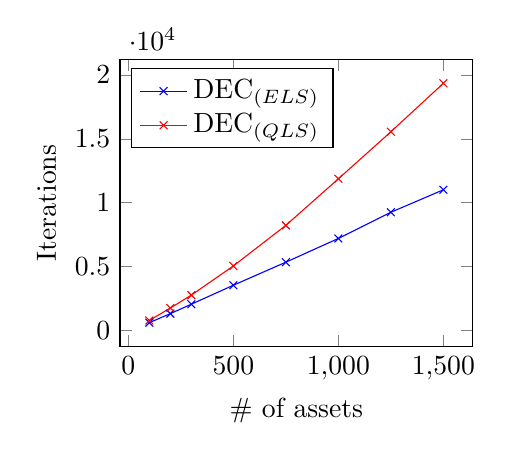
\begin{tikzpicture}
\begin{axis}[%
xlabel={\# of assets},
ylabel={Iterations},
legend pos=north west,
ylabel near ticks,
width=.5\textwidth
]
\addplot [color=blue,solid,mark=x,mark options={solid}]
  table[row sep=crcr]{%
%50	242\\
%75	379\\
100	609 \\
200	1315 \\
300	2053 \\
500	3538\\
750	5343 \\
1000	7200\\
1250	9251\\
1500    11011\\
};

\addplot [color=red,solid,mark=x,mark options={solid}]
 table[row sep=crcr]{%
%%50	309    \\
%%75	483    \\
100	782    \\
200	1754		\\
300	2763		\\
500	5048		\\
750	8225		\\
1000	 11871	\\
1250	 15552	\\
1500	 19347\\
};

\addlegendentry{DEC$_{(ELS)}$}
\addlegendentry{DEC$_{(QLS)}$}
\end{axis}
\end{tikzpicture}
}
}
\caption{Comparison of performances using $\epsilon = 10^{-10}$ in (\ref{eq:stop}) with box constraints defined in (\ref{eq:classicalbox})}
\end{figure}

\subsubsection{Convergence to a Risk Parity solution}
In this section we evaluate the probability to converge to a critical point $(x^*,y^*)$ that is also a Risk Parity solution, i.e. that satisfies 
\begin{equation}\label{eq:reseps}
\max_i \left| \frac{RC_i}{\mathcal{R}(x^*,y^*)} - \frac{1}{n} \right| < 10^{-6}
\end{equation}
where $RC_i$ is the risk contribution of the asset $i$ and ${\mathcal{R}(x^*,y^*)}$ is the total risk of the invested portfolio. Equation (\ref{eq:reseps}) express the fact that the (normalized) max deviation from Risk Parity of the solutions is less than $10^{-6}$. In Figure (\ref{fig:convergence1}) and (\ref{fig:convergence2}) we compare the probability to reach a Risk Parity solution for both the decomposition algorithm (with inexact and exact line search) and SNOPT, using different choices of the starting point $x^0$. 

\begin{figure}
\makebox[\textwidth][c]{
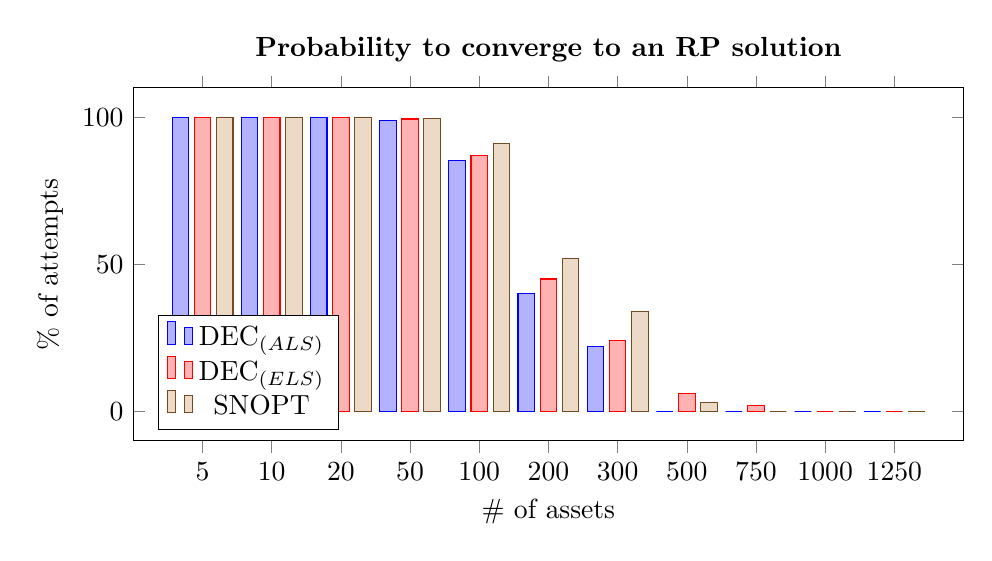
\begin{tikzpicture}
\begin{axis}[%
ybar,
width=\textwidth,
height=0.5\textwidth,
xlabel={\# of assets},
ylabel={\% of attempts},
ylabel near ticks,
legend pos=south west,
symbolic x coords = {5,10,20,50,100,200,300,500,750,1000,1250},
bar width=6pt,
xtick=data,
title=\textbf{Probability to converge to an RP solution}
]
\addplot coordinates { 
(5,100)         
(10,100)
(20,100)
(50,99)
(100,85.4)
(200,40)
(300,22)
(500,0)
(750,0)
(1000,0)
(1250,0)
 };
 
 \addplot coordinates { 
(5,100)         
(10,100)
(20,100)
(50,99.4)
(100,87)
(200,45)
(300,24)
(500,6)
(750,2)
(1000,0)
(1250,0)
 };
 
  \addplot coordinates { 
(5,100)         
(10,100)
(20,100)
(50,99.5)
(100,91.2)
(200,52)
(300,34)
(500,3)
(750,0)
(1000,0)
(1250,0)
 };

\addlegendentry{DEC$_{(ALS)}$ }
\addlegendentry{DEC$_{(ELS)}$}
\addlegendentry{SNOPT}
\end{axis}
\end{tikzpicture}
}
\caption{Probability to converge to a Risk Parity solution using $x^{0}_i = 1/n \quad \forall i$ for the decomposition algorithm (DEC) (with ALS or ELS) and SNOPT.}
\label{fig:convergence1}
\vspace{2em}
\makebox[\textwidth][c]{
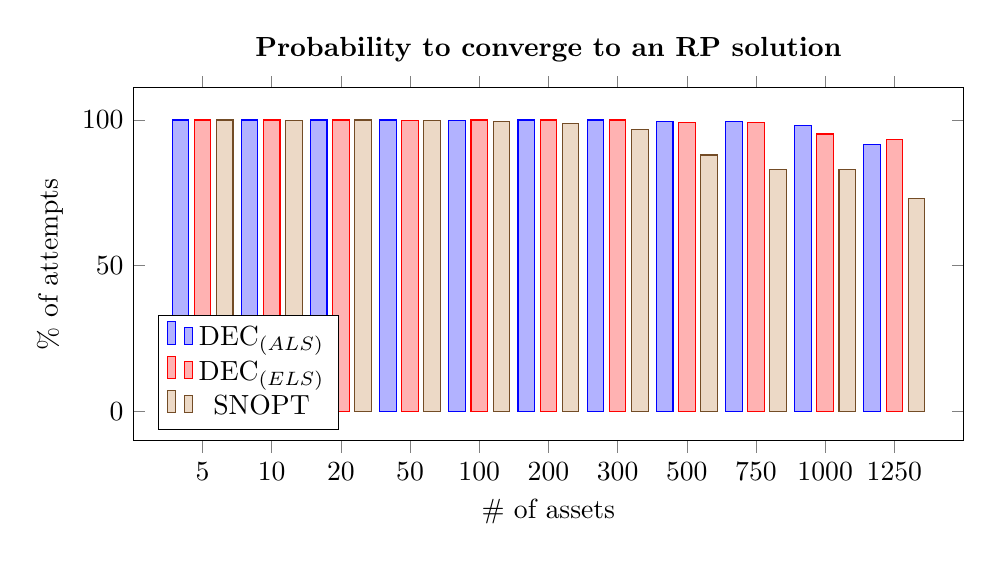
\begin{tikzpicture}
\begin{axis}[%
ybar,
width=\textwidth,
height=0.5\textwidth,
xlabel={\# of assets},
ylabel={\% of attempts},
ylabel near ticks,
legend pos=south west,
symbolic x coords = {5,10,20,50,100,200,300,500,750,1000,1250},
bar width=6pt,
xtick=data,
ymin=-10,
title=\textbf{Probability to converge to an RP solution}
]
\addplot coordinates { 
(5,100)         
(10,100)
(20,100)
(50,100)
(100,99.9)
(200,100)
(300,100)
(500,99.5)
(750,99.5)
(1000,98)
(1250,91.5)
 };
 
 \addplot coordinates { 
(5,100)         
(10,100)
(20,100)
(50,99.9)
(100,100)
(200,100)
(300,100)
(500,99.2)
(750,99.2)
(1000,95.2)
(1250,93.2)
 };
 
  \addplot coordinates { 
(5,100)         
(10,99.9)
(20,100)
(50,99.9)
(100,99.6)
(200,98.8)
(300,96.6)
(500,88)
(750,83)
(1000,83)
(1250,73)
 };

\addlegendentry{DEC$_{(ALS)}$ }
\addlegendentry{DEC$_{(ELS)}$}
\addlegendentry{SNOPT}
\end{axis}
\end{tikzpicture}
}
\caption{Probability to converge to a Risk Parity solution using $x^{0}= [1, 0, .., 0]$ for the decomposition algorithm (DEC) (with ALS or ELS) and SNOPT.}
\label{fig:convergence2}
\end{figure}

%\begin{table}
%\centering
%\begin{tabular}{ c | c | c | c }
%n &  G-S$_{(ALS)}$ & G-S$_{(ELS)}$  & SNOPT \\\hline
%5    & 100.0\% & 100.0\% & 100.0\%\\\hline
%10   & 100.0\% & 100.0\% & 100.0\%\\\hline
%20   & 100.0\% & 100.0\% & 100.0\%\\\hline
%50   & 99.0\%  & 99.4\%  & 99.5\%\\\hline
%100  & 85.4\%  & 87.0\%  & 91.2\%\\\hline
%200  & 40.0\%  & 45.0\%  & 52.0\%\\\hline
%300  & 22.0\%  & 24.0\%  & 34.0\%\\\hline
%500  & 0.0\%   & 6.0\%   & 3.0\%\\\hline
%750  & 0.0\%   & 2.0\%   & 0.0\%\\\hline
%1000 & 0.0\%   & 0.0\%   & 0.0\%\\\hline
%1250 & 0.0\%   & 0.0\%   & 0.0\%\\\hline
%\end{tabular}
%\caption{Probability to converge to a Risk Parity solution using $x^{0}_i = 1/n \quad \forall i$}
%\label{tab:first}
%\end{table}
%
%
%\begin{table}
%\centering
%\begin{tabular}{ c | c | c | c}
%n &  G-S$_{(ALS)}$ & G-S$_{(ELS)}$  & SNOPT \\\hline
%5    & 100.0\%  & 100.0\% & 100.0\%\\\hline
%10   & 100.0\%  & 100.0\% & 99.9\%\\\hline
%20   & 100.0\%  & 100.0\%  & 100.0\%\\\hline
%50   & 100.0\%  & 99.9\%  & 99.9\%\\\hline
%100  & 99.9\%   & 100.0\%  & 99.6\% \\\hline
%200  & 100.0\%  & 100.0\%  & 98.8\% \\\hline
%300  & 100.0\%  & 100.0\%  & 96.6\% \\\hline
%500  & 99.5\%   & 99.2\%   & 88.0\%\\\hline
%750  & 99.5\%   & 99.2\%  & 83.0\%\\\hline
%1000 & 98.0\%   & 95.2\%  & 83.0\%\\\hline
%1250 & 91.5\%   & 93.2\%  & 73.0\%\\\hline
%\end{tabular}
%\caption{Probability to converge to a Risk Parity solution using $x^{0}= [1, 0, .., 0]$}
%\label{tab:second}
%\end{table}

\subsubsection{On the choosing of starting point}
From Figures (\ref{fig:convergence1}) and (\ref{fig:convergence2}) it is clear that the choice of the starting point $x^0$ strongly affects the probability of the algorithms to reach a Risk Parity solution. More in details, in Figure (\ref{fig:convergence1}) we use a fully dense starting point while in Figure (\ref{fig:convergence2}) we use the most sparse feasible starting point. In Figure (\ref{fig:sparsity}) we measure the probability to reach a Risk Parity solution varying the sparsity of the initial guess $x^0$, i.e. the percentage of components of $x^0$ fixed to 0. In the left side of Figure (\ref{fig:sparsity}) we use an equally distributed starting point:
\begin{equation}
x^{0} = [x^{0}_0, x^{0}_1, .. ,  x^{0}_k, x^{0}_{k+1} .., x^{0}_n] = [\frac{1}{k}, \frac{1}{k}, .., \frac{1}{k}, 0, .., 0]
\end{equation}
In the right side of Figure (\ref{fig:sparsity}) we use a random distributed starting point:
\begin{equation}
\begin{aligned}
&a^{0} = [r_0, r_1, ..,r_k, 0, .., 0] \qquad \text{where} \quad r_i \sim \mathcal{U}[0,1]\\
&x^0 = \frac{a^{0}}{\mathds{1}^T a^0}
\end{aligned}
\end{equation}

\begin{figure}
\makebox[\textwidth][c]{
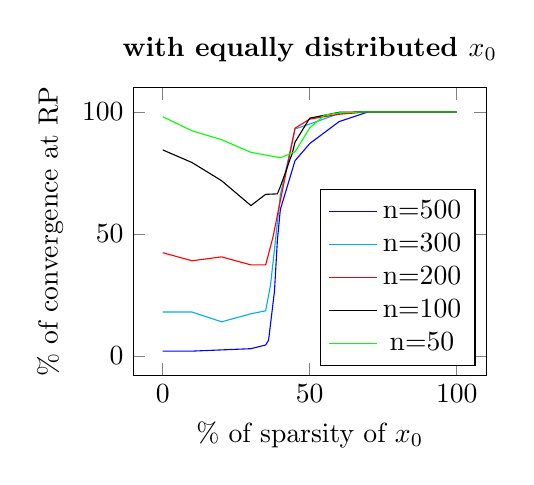
\begin{tikzpicture}
\begin{axis}[%
xlabel={\% of sparsity of $x_0$},
ylabel={\% of convergence at RP},
scaled y ticks=false,
width=0.5\textwidth,
legend pos=south east,
title=\textbf{with equally distributed $x_0$}
]

\addplot [color=blue,solid,mark=none,mark options={solid}]
  table[row sep=crcr]{%
0 2 \\
10 2 \\
20 2.5 \\
30 3 \\
35 4.5 \\
36 6.5
37 14.5 \\
38 26.5 \\
39 47.5 \\
40 60 \\
45 80\\
50 87 \\
60 96 \\
70 100 \\
80 100 \\
90 100 \\
100 100 \\
};

\addplot [color=cyan,solid,mark=none,mark options={solid}]
  table[row sep=crcr]{%
0 18\\
10 18 \\
20 14 \\
30 17.3 \\
35 18.5 \\
36.67 29.1 \\
38.3 47 \\
40 66 \\
45 93 \\
50 95 \\
60 99.3 \\
70 100 \\
80 100 \\
90 100 \\
100 100\\
};

\addplot [color=red,solid,mark=none,mark options={solid}]
  table[row sep=crcr]{%
0 42.3 \\
10 39 \\
20 40.6 \\
30 37.3 \\
35 37.3 \\
37.5 48.7 \\
38.5 54.7 \\
40 63.6 \\
45 93.3 \\
50 97 \\
60 99 \\
70 100 \\
80 100 \\
90 100 \\
100 100\\
};

\addplot [color=black,solid,mark=none,mark options={solid}]
  table[row sep=crcr]{%
0 84.4 \\
10 79.2 \\
20 71.8 \\
30 61.6 \\
35 66.2 \\
39 66.4 \\
40 69.4 \\
42 76 \\
43 79.6 \\
44 82.8\\
45 87.6 \\
50 97.4 \\
60 99.8 \\
70 100 \\
80 100 \\
90 100 \\
100 100\\
};

\addplot [color=green,solid,mark=none,mark options={solid}]
  table[row sep=crcr]{%
0 98 \\
10 92.2 \\
20 88.6\\
30 83.4 \\
40 81.2 \\
45 83.6 \\
50 93.4 \\
55 98.6 \\
60 99.6 \\
70 100 \\
80 100 \\
90 100 \\
100 100 \\
};
\addlegendentry{n=500}
\addlegendentry{n=300}
\addlegendentry{n=200}
\addlegendentry{n=100}
\addlegendentry{n=50}
\end{axis}
\end{tikzpicture}

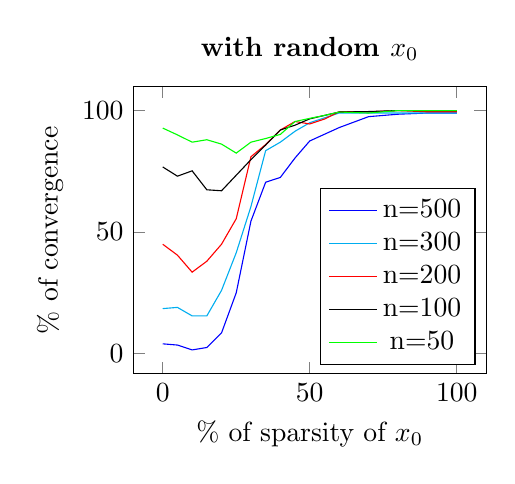
\begin{tikzpicture}
\begin{axis}[%
width=0.5\textwidth,
xlabel={\% of sparsity of $x_0$},
ylabel={\% of convergence},
legend pos=south east,
title=\textbf{with random $x_0$}
]

\addplot [color=blue,solid,mark=none,mark options={solid}]
  table[row sep=crcr]{%
0  4.0 \\
5  3.5 \\
10 1.5 \\
15 2.5 \\
20 8.5 \\
25 25.0 \\
30 54.5 \\
35 70.5 \\
40 72.5 \\
45 80.5 \\
50 87.5 \\
60 93 \\
70 97.5 \\
80 98.5 \\
90 99.0 \\
100 99.0 \\
};

\addplot [color=cyan,solid,mark=none,mark options={solid}]
  table[row sep=crcr]{%
0 18.5 \\
5 19.0 \\
10 15.5 \\
15 15.5 \\
20 26.0 \\
25 41.5 \\
30 60.5 \\
35 83.5 \\
40 87.0 \\
45 91.5 \\
50 95.0 \\
60 99.0 \\
90 99.0 \\
100 99.0 \\
};

\addplot [color=red,solid,mark=none,mark options={solid}]
  table[row sep=crcr]{%
0 45 \\
5 40.5 \\
10 33.5 \\
15 38.0 \\
20 45.0 \\
25 55.5 \\
30 81.0 \\
35 86.0 \\
40 92.0 \\
45 95.5 \\
50 94.5 \\
55 96.5 \\
60 99.5 \\
70 99.5 \\
80 100 \\
90 99.5 \\
100 99.5 \\
};

\addplot [color=black,solid,mark=none,mark options={solid}]
  table[row sep=crcr]{%
0 76.8 \\
5 73 \\
10 75.2 \\
15 67.4 \\
20 67 \\
25 73.4 \\
30 79.8 \\
35 85.8 \\
40 92 \\
45 94 \\
50 96.6 \\
55 98 \\
60 99.4 \\
70 99.6 \\
80 100 \\
90 100 \\
100 100 \\
};

\addplot [color=green,solid,mark=none,mark options={solid}]
  table[row sep=crcr]{%
0 92.8\\
5 90 \\
10 87.0 \\
15 88.0 \\
20 86.2\\
25 82.5 \\
30 87.0 \\
35 88.5 \\
40 90.2 \\
45 95.5 \\
50 96.8 \\
55 98.0 \\
60 99.4 \\
70 99.0 \\
80 100 \\
90 100 \\
100 100\\
};


\addlegendentry{n=500}
\addlegendentry{n=300}
\addlegendentry{n=200}
\addlegendentry{n=100}
\addlegendentry{n=50}
\end{axis}
\end{tikzpicture}
}

\caption{Percentage of computations that find an RP solution, varying the sparsity of the initial guess $x^0$, for different number of assets $n$}
\label{fig:sparsity}
\end{figure}


